\documentclass{standalone}
% \usepackage[margin=0.25in]{geometry}
\usepackage{pgfplots}
\pgfplotsset{width=10cm,compat=1.9}

% \usepgfplotslibrary{external}
% \tikzexternalize

\begin{document}

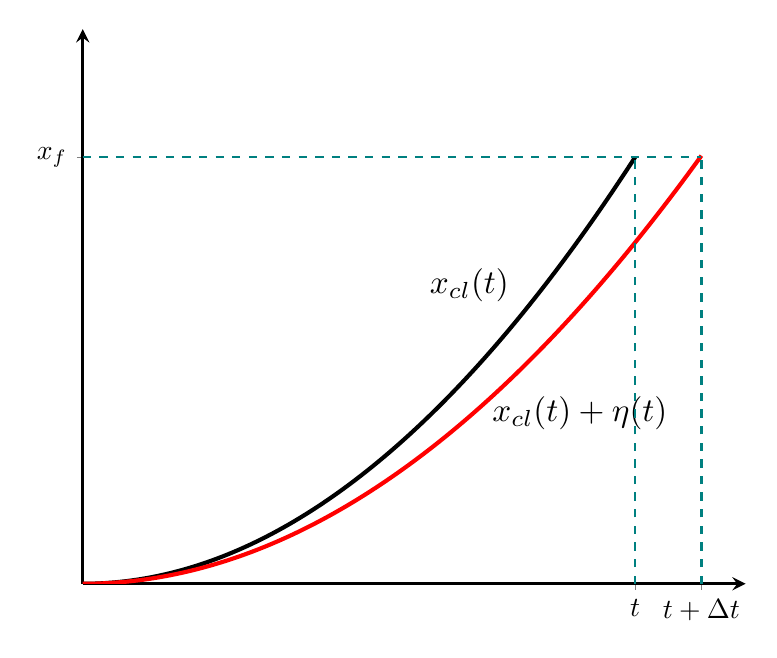
\begin{tikzpicture}
    \begin{axis}[
        axis lines = left,        % xlabel = \(t\),
        % ylabel = {\(x\)},
        outer axis line style={line width=1.1pt},
        xmin = 0,
        xmax = 1.2,
        ymin = 0,
        ymax = 1.3,
        xtick={1, 1.12}, 
        xticklabels = {\(t\), \(t+\Delta t\)},
        ytick={1, 2},
        yticklabels = {\(x_f\), \(a\)},
    ]    
    \addplot [
    domain=0:1, 
    samples=100, 
    color=black,
    line width=1.5pt,
    ]
    {x^2};
    \addplot [
    domain=0:1.12, 
    samples=100, 
    color=red,
    line width=1.5pt,
    ]
    {0.8*x^2};
    \node at (axis cs:0.7, 0.7) [scale=1.2] {$x_{cl}(t)$};
    \node at (axis cs:0.9, 0.4) [scale=1.2] {$x_{cl}(t)+ \eta(t)$};
    \draw[thick, teal, dashed] (axis cs:0.0, 1.0) -- (axis cs:1.12 ,1.0);
    \draw[thick, teal, dashed] (axis cs:1.0, 0.0) -- (axis cs:1.0 ,1.0);
    \draw[thick, teal, dashed] (axis cs:1.12, 0.0) -- (axis cs:1.12 ,1.0);
    \end{axis}
    \end{tikzpicture}
\end{document}